\chapter{Desenvolvemento}
\label{cap:desarrollo}

% TFG BREVE: Es conveniente comenzar el capítulo un un par de párrafos que explique su contenido. Por ejemplo: "En este capítulo se presenta en desarrollo del proyecto realizado. Comenzaremos explicando las tecnologías utilizadas para, posteriormente, detallar ...."
Neste capítulo preséntase o desenvolvemento do proxecto realizado. Comenzaremos cas eleccións tecnolóxicas que se tomaron para acadar o mellor resultado que cumpra os requirimentos recollidos. Despois detallaremos o proceso de desenvolvemento explicando a resolución das problemáticas atopadas e a implementación dos diferentes prototipos ata chegar ao resultado conseguido.  

\section{Tecnologías}
% En el TFG se suele poner un capítulo completo dedicado a las tecnologías empleadas, pero en el TFG BREVE se hará en esta sección. Se pretende resumir las tecnologías y explicar por qué se han elegido. Hay que evitar hacer copy-paste de web. Además, es importante poner referencias bibliográficas utilizando este formato: \cite{ErlangBook,ErlangWebBook}. 
Para a implementación do sistema hardware que fai de teclado de piano o microcontrolador empregado foi o ESP32 como o da figura \ref{fig:esp32}. Este microcontrolador é un SoC e é moi valorado tanto no entorno educativo coma no empresarial pola súa relación prezo-prestacións. Mantendo un prezo por debaixo dos 10 euros ofrece un sistema de baixo consumo, con unha cantidade notable de pins para o seu reducido tamaño, soporte para as contornas de desenvolvemento de Arduino e con outras contornas como Thonny, a utilizada nas sesións de prácticas da materia; e como factor máis destacable, Wifi e Bluetooth integrados sen necesidade de un módulo a maiores\cite{ESP32MX}. Ademais destas características a elección foi motivada tamén porque é a placa utilizada en algunhas sesións de prácticas da materia.
Para a súa programación empregaremos empregaremos Micropython, unha implementación de Python 3 orientada a microcontroladores \cite{MicroPython}. Neste caso tamén usamos esta contorna na materia. Ademais, permítenos programar de forma moi flexible e cómoda cunha linguaxe de moi alto nivel co que xa estou familiarizado. Como o programa a implementar é sinxelo e non empregamos unha gran cantidade de recursos podémonos permitir utilizar este entorno menos eficiente pero máis cómodo co que traballar.

\begin{figure}[hp!]
  \centering
  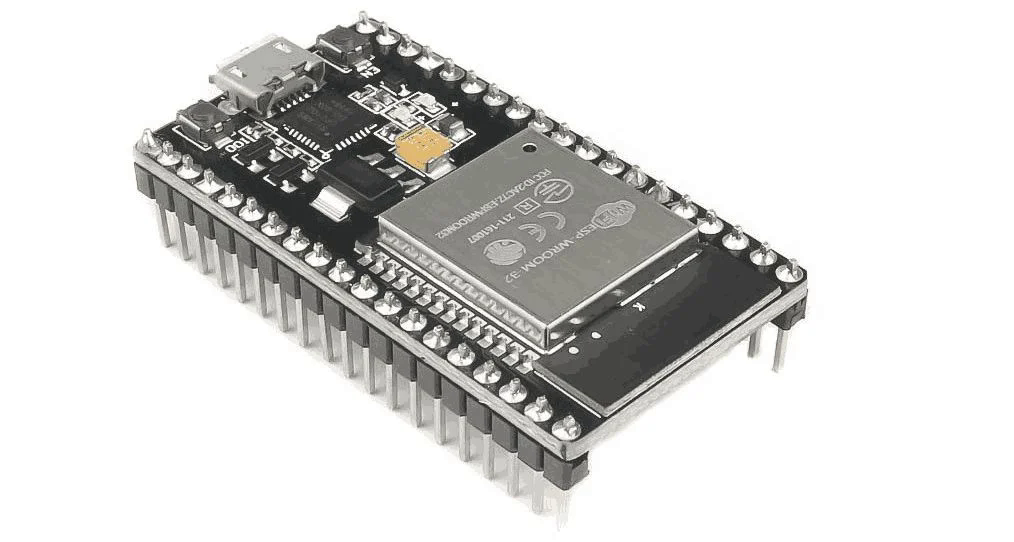
\includegraphics[width=0.75\textwidth]{imaxes/ESP32.png}
  \caption{Imaxe dun ESP32}
  \label{fig:esp32}
\end{figure}

\newline{}\newline{}
Para o desenvolvemento da aplicación principal a necesidade de cumprir cuns estándares de accesibilidade importantes fixeron que a elección da plataforma para desenvolver a vista fose unha tecnoloxía web. A web é das contornas con máis ferramentas para as persoas con necesidades de accesibilidade específicas. Iniciativas e estándares como Web Accessibility Initiative \cite{WAI} do W3C fan que as utilidades para estas persoas sexan numerosas e o traballo dos programadores mínimo. Frente á web, outras plataformas non teñen tan desenvoltos estes aspectos.

Para poder interactuar co sistema operativo para o control do sistema hardware requirimos que esta vista web se execute fóra da contorna illada dun navegador. Existen varias tecnoloxías que nos permiten facer isto. A máis importante sen dúbida é Electron \cite{Electron}. Esta tecnoloxía empaqueta o navegador Chromium e a contorna de execución de Javascript Nodejs para obter unha plataforma para aplicacións multiplataforma sen código específico de cada plataforma e permitindo compartir unha vista entre a versión web e a versión de escritorio ou móbil. Úsase por exemplo, en VSCode, en Discord ou en Microsoft Teams. 

A plataforma finalmente elixida é unha alternativa a esta última ferramenta, pero que soluciona un dos maiores problemas desta. Esta alternativa é Tauri \cite{Tauri}.
Tauri permite crear aplicacións multiplataforma sen necesidade de ter empaquetados moi pesados. Mentres cada aplicación que utiliza Electron empaqueta o seu propio Chromium e Nodejs, Tauri utiliza a vista web nativa do sistema operativo e o seu núcleo é un binario codificado en Rust \cite{Rust} moi livián, comunicados mediante o paso de mensaxes entre diferentes procesos, como se mostra na figura \ref{fig:TauriIPC}. Isto permite pasar de tamaños de aplicacións da orde de centos de megabytes a soamente uns poucos megabytes. Isto tamén produce inconvenientes, xa que ao depender da vista web nativa, esta non será totalmente igual en todos os sistema, debido ás diferentes implementacións e versións dos motores de renderizado que utiliza cada sistema operativo. Por exemplo, en Windows utilízase o motor WebView2 (baseado en Edge que á súa vez basease en Chromium), mentres que en macOS emprega WebKit, e en Linux úsase WebKitGTK. A pesar deste problema, elixín esta opción ao ser este un problema menor que tamén pasa na web entre diferentes navegadores e ao ser o beneficio maior ás desventaxas. 

\begin{figure}[hp!]
  \centering
  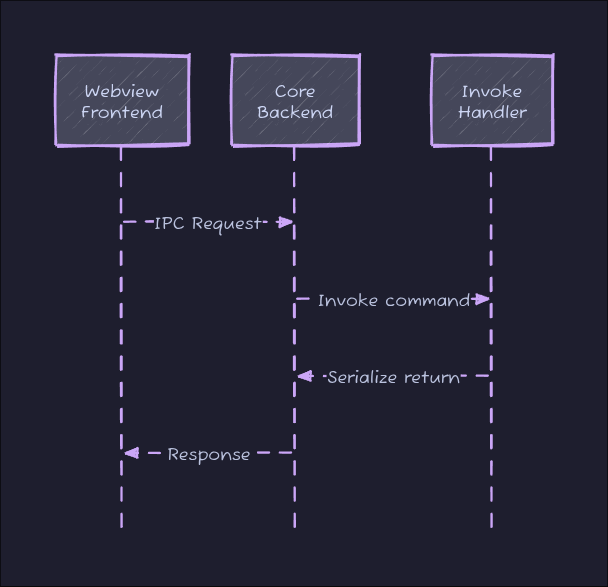
\includegraphics[width=0.75\textwidth]{imaxes/TauriIPC.png}
  \caption{Diagrama da comunicación entre procesos de Tauri}
  \label{fig:TauriIPC}
\end{figure}

Para codificar a vista usei a popular librería de UI desenvolta por Meta, React \cite{React}. Esta opción moi usada tanto a nivel nacional como internacional permítenos desenvolver aplicacións reactivas de xeito sinxelo e moi cómodo para o programador. Ademais, utilicei a linguaxe Typescript, que transpila a Javascript, para ter unha mellor experiencia de desenvolvemento e acadar un produto máis facilmente mantible ao longo do tempo.

Para a manipulación do son utilízase a librería de manipulación de son Rodio \cite{Rodio}, que nos permite reproducir son de forma multiplataforma.

Para o control do porto serie para a comunicación co sistema hardware utilízase a librería serialport-rs \cite{Serialport}, que nos permite traballar co porto serie abstraendo as peculiaridades de cada sistema operativo. 


\section{Desarrollo}
% En el TFG suele haber varios capítulos para explicar el desarrollo realizados. Aquí lo haremos en un solo capítulo.

% En el caso de proyectos con microcontroladores, se debe indicar claramente el montaje. 

% En caso de incluir figuras, deben referenciarse de esta forma "la figura~\ref{fig:exemplo} ". Todas las figuras deben estar referenciadas en el texto.
% Se recomienda poner todas las figuras en el directorio \texttt{imaxes}.
O primeiro prototipo do proxecto consistiu en facer unha aplicación na que se puidese reproducir o son dun elefante cando ao pulsar as teclas do teclado do ordenador. Esta primeira aproximación permitiu primeiro desenvolver o sistema de procesado de son antes que o resto do proxecto. Ademais disto, permitiume familiarizarme con Tauri e o seu paso de mensaxes entre o proceso que executa a vista web e o proceso que executa o núcleo en Rust. Como vemos nas figuras \ref{fig:playNote} e \ref{fig:invokePlayNote} para dende a vista web podemos invocar comandos que se executarán no núcleo da aplicación. 

\begin{figure}[hp!]
  \centering
  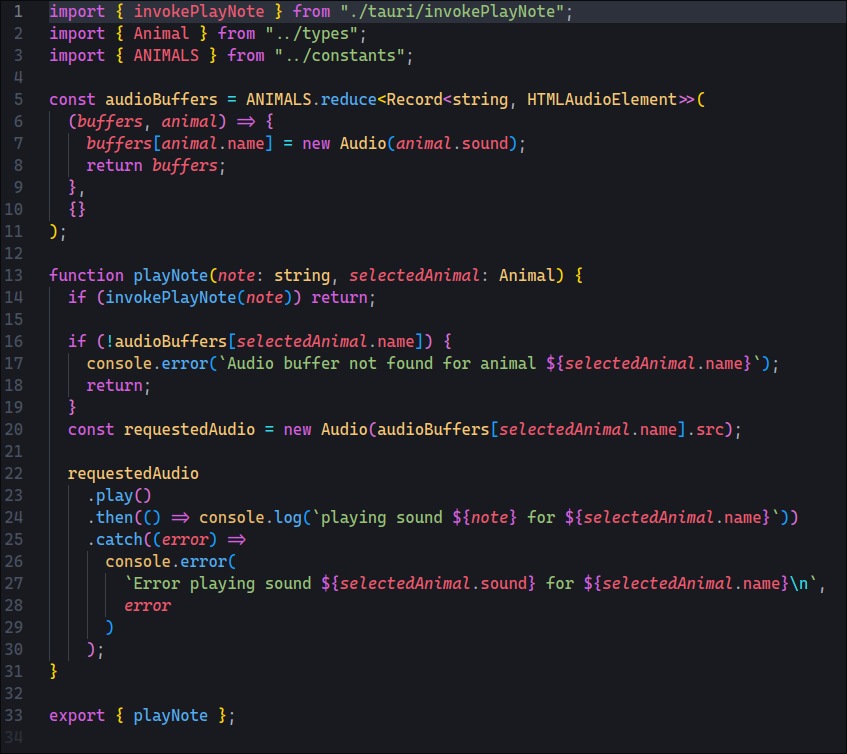
\includegraphics[width=0.75\textwidth]{imaxes/playNote.png}
  \caption{Código correspondente á reprodución de son no navegador}
  \label{fig:playNote}
\end{figure}

\begin{figure}[hp!]
  \centering
  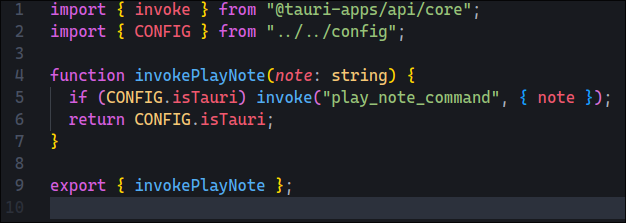
\includegraphics[width=0.75\textwidth]{imaxes/invokePlayNote.png}
  \caption{Código correspondente á invocación dun comando de Tauri}
  \label{fig:invokePlayNote}
\end{figure}

O sistema de procesado de son atópase no núcleo da aplicación. Tomei decisión de deseño en vez de usar a API do navegador para reproducir son porque desta forma sería máis fácil integrar o sistema á hora de reproducir son demandado polo sistema hardware. Da outra maneira habería que comunicar os mensaxes do sistema hardware ca vista web, complicando a arquitectura. A outra posible desvantaxe sería unha maior dificultade de modificar este son usando as API do navegador.

Un dos primeiros obstáculos que se atoparon foi a natureza bloqueante da reprodución de son. Para solucionar isto, a solución foi executar a reprodución noutro fío secundario, que podemos utilizar de forma moi sinxela grazas ás funcións asíncronas de Rust, como vemos na figura \ref{fig:playNoteCommand}. Tauri utiliza Tokio, un runtime asíncrono de Rust que implementa "fíos verdes", permitindo executar bloques asíncronos con gran facilidade. Estes fíos verdes\cite{GreenThread} consisten en executar en fíos xestionados por un runtime (neste caso Tokio) ou unha máquina virtual. En vez de crear un fío do sistema operativo para cada operación, o sistema ten unha piscina de fíos que administra dun xeito similar ao bucle de eventos de Javascript.

\begin{figure}[hp!]
  \centering
  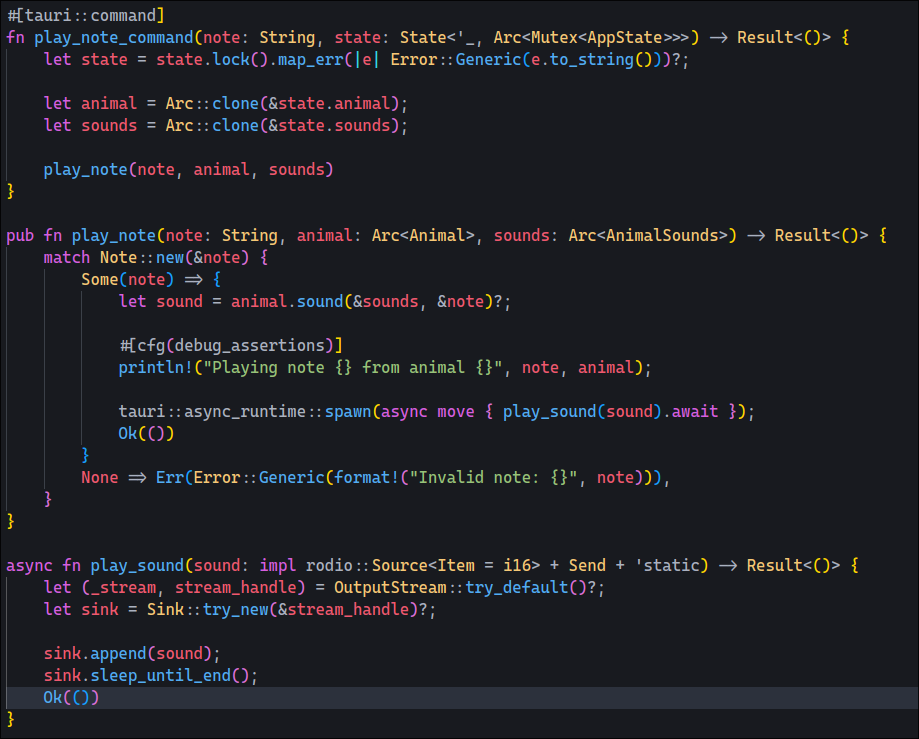
\includegraphics[width=0.75\textwidth]{imaxes/playNoteCommand.png}
  \caption{Código correspondente á execución do son, dende un fío secundario}
  \label{fig:playNoteCommand}
\end{figure}

Para o procesamento do son para soar como unha nota musical, tomando como base o son dun animal gardado nunha pista de son wav o que facemos e aplicarlle unha aceleración ao son seleccionado. Dependendo da nota desexada acelérase máis. Canto máis aguda sexa a nota máis debemos acelerar. Esto faise seguindo o sistema do temperamento igual de 12 tons \cite{Semitone}. Cada semitón representa un incremento de frecuencia equivalente á raíz doceava de 2, polo que cada semitón representa un incremento de frecuencia (acelerando) equivalente á raíz doceava de 2, polo que para modificar a altura dun son orixinal sen alterar o seu timbre nin a súa duración relativa, multiplícase a súa frecuencia polo factor 
\[
f = f_0 \cdot 2^{\frac{n}{12}}
\]
onde n é o número de semitóns de diferenza respecto á nota base.

\begin{figure}[hp!]
  \centering
  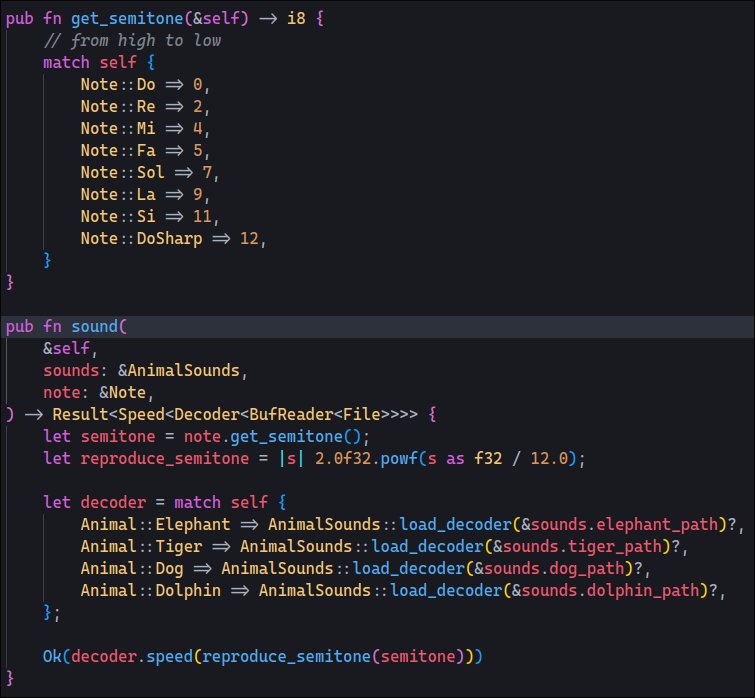
\includegraphics[width=0.75\textwidth]{imaxes/semitone.png}
  \caption{Código correspondente á execución do son}
  \label{fig:semitone}
\end{figure}

O seguinte problema que se presentou foi que os arquivos soamente se podían reproducir executando a aplicación en modo desenvolvemento. Para facer que Tauri inclúa na aplicación final os arquivos, debemos facer referencia a eles, en vez a través das rutas relativas ao proxecto, a través do resolvente de camiños de Tauri, como se amosa na figura \ref{fig:resolvePath}. Desta forma, os sons son incluídos na versión final da aplicación.

\begin{figure}[hp!]
  \centering
  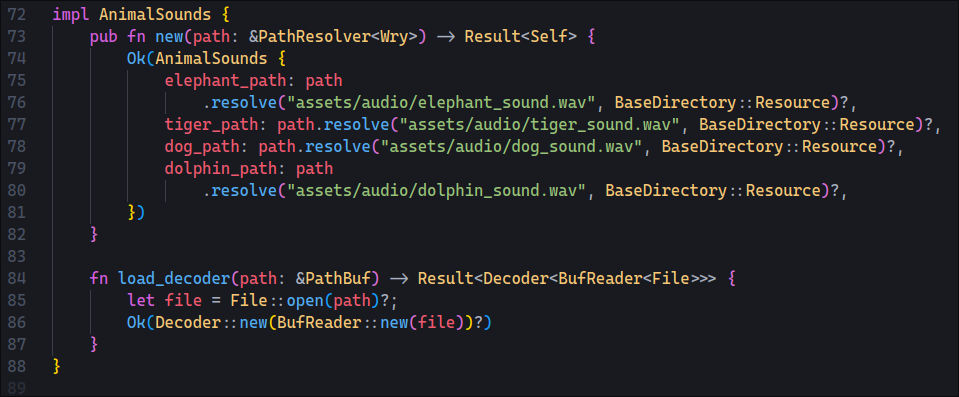
\includegraphics[width=0.75\textwidth]{imaxes/resolvePath.png}
  \caption{Código amosando a resolución de camiños}
  \label{fig:resolvePath}
\end{figure}

Unha vez que a reprodución e procesamento de son funcionaron de forma correcta no ordenador comecei a traballar na implementación do teclado baseado nun microcontrolador, co deseño que vemos na figura \ref{fig:microcontrolador}. O sistema inicial soamente incluía un só botón pero o seu funcionamento é o mesmo, usando os pins 26 para a nota re, o 25 para a nota sol e o 33 para a nota si. Como vemos na figura \ref{fig:micropython}, o código consiste en enviar a través do porto serie o nome da nota correspondente á tecla premida.

\begin{figure}[hp!]
  \centering
  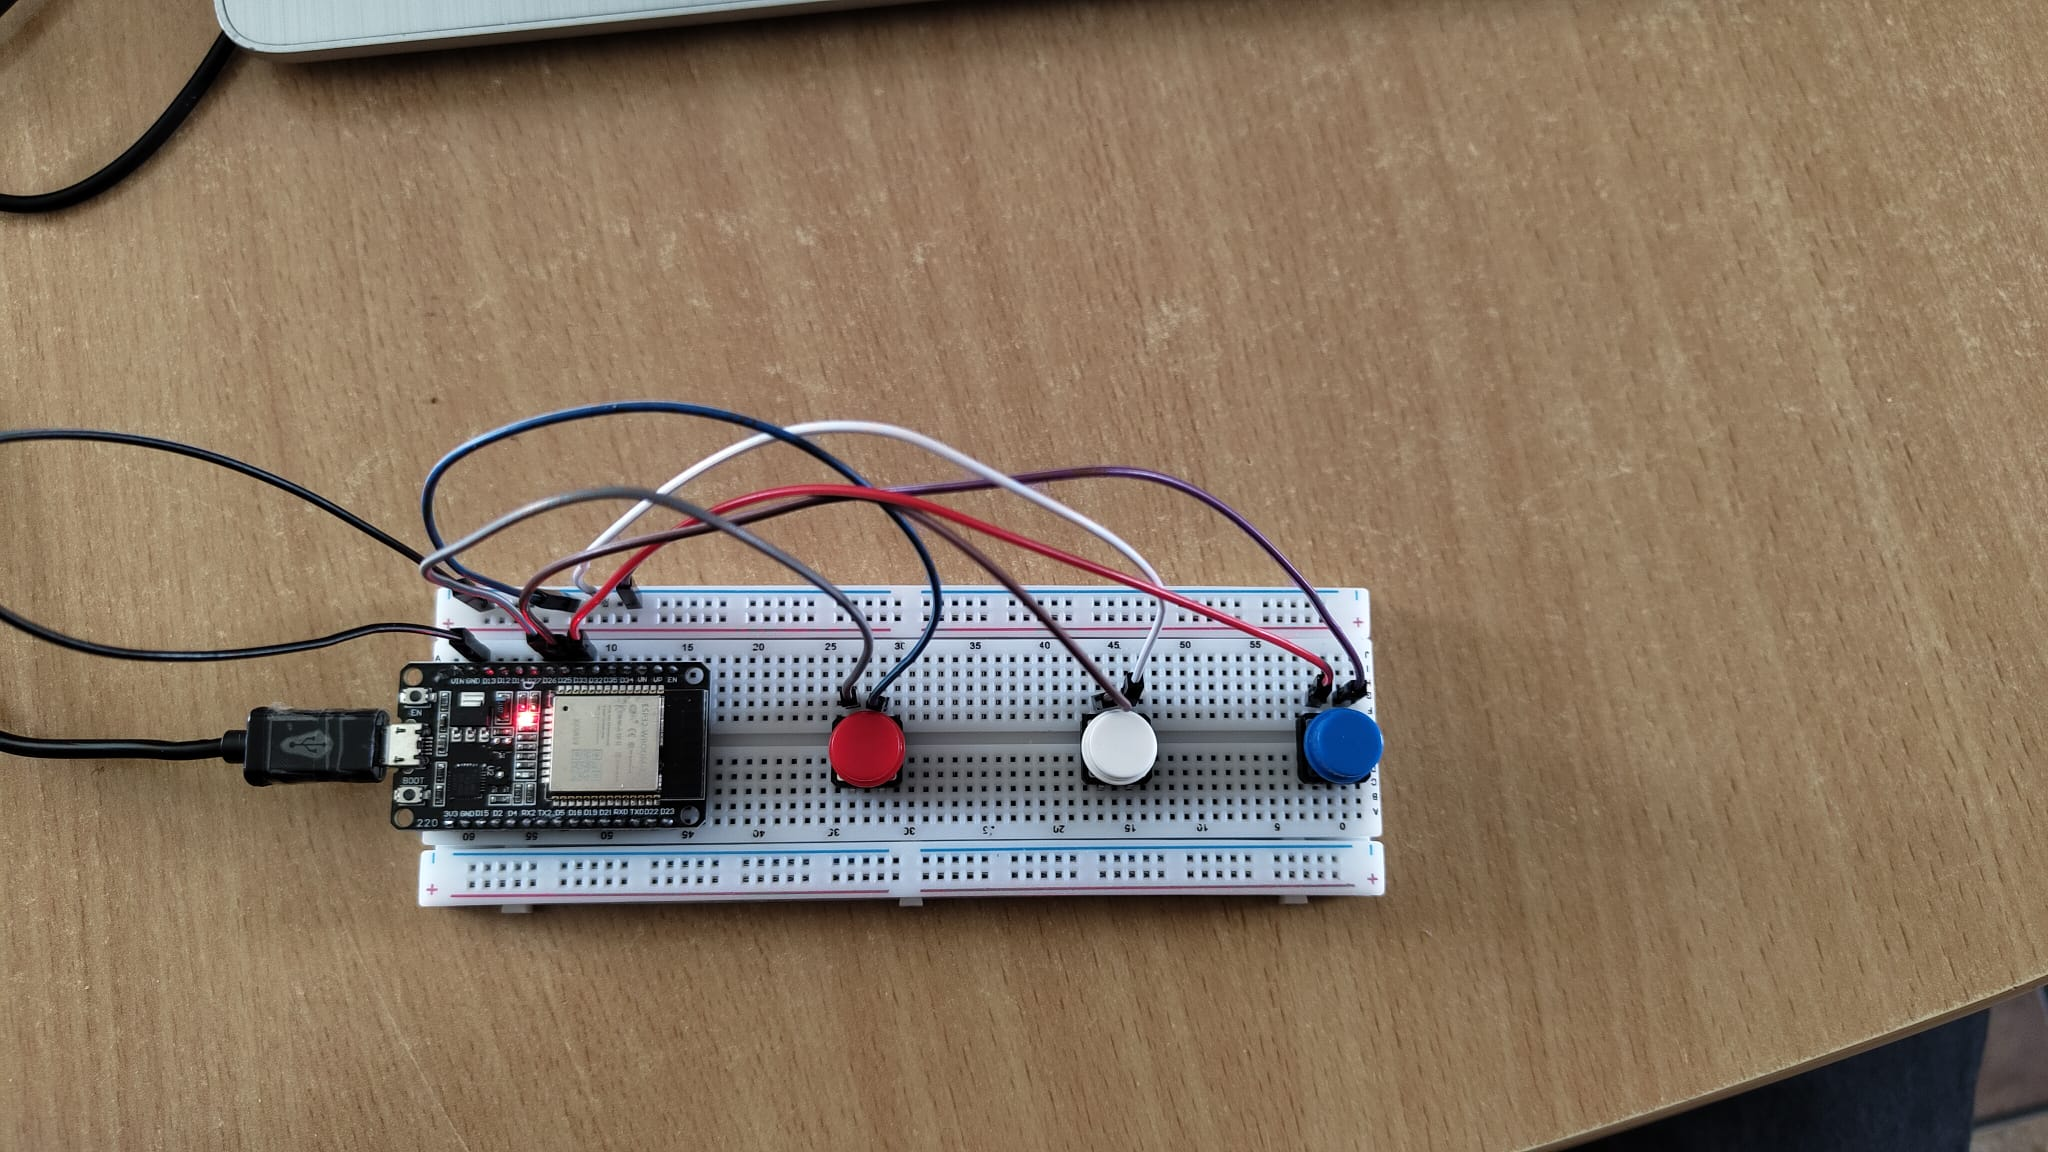
\includegraphics[width=0.75\textwidth]{imaxes/microcontrolador.jpeg}
  \caption{Deseño do sistema hardware}
  \label{fig:microcontrolador}
\end{figure}

\begin{figure}[hp!]
  \centering
  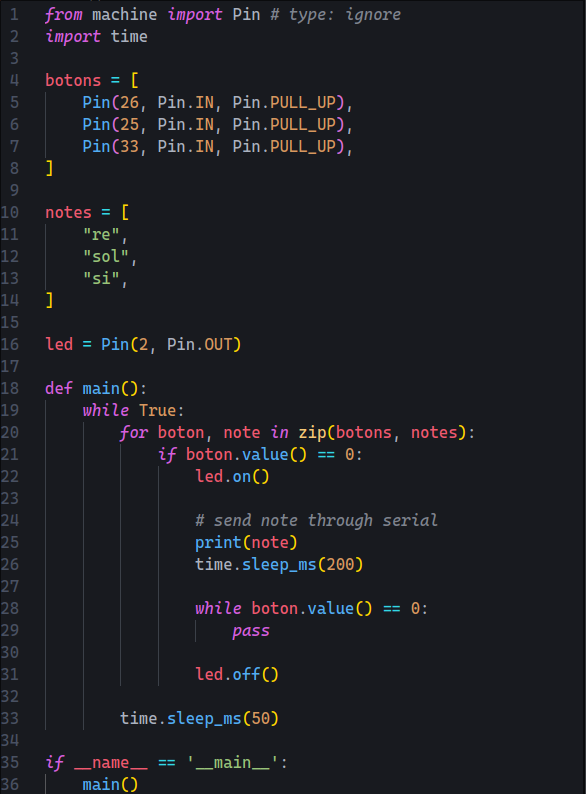
\includegraphics[width=0.75\textwidth]{imaxes/micropython.png}
  \caption{Código de Micropython do teclado}
  \label{fig:micropython}
\end{figure}

O seguinte paso foi a lectura do porto serie dende a aplicación para a reprodución da nota usando a librería \cite{Serialport}. Para implementar a lectura usouse un fío específico que lee de forma continua o porto serie se hai algún dispoñible. Cando se realiza unha lectura no porto, envíase a través dun canal ao fío principal para poder reproducir o son, como vemos na figura \ref{fig:sender}.  

\begin{figure}[hp!]
  \centering
  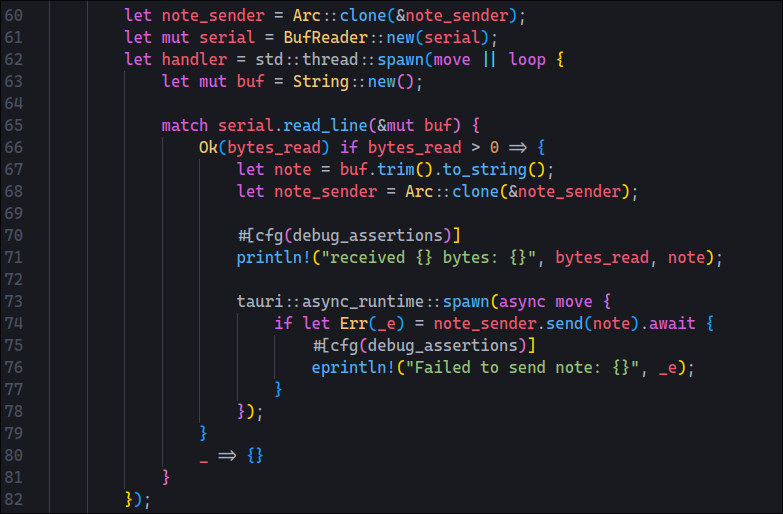
\includegraphics[width=0.75\textwidth]{imaxes/sender.png}
  \caption{Lectura e envío das notas do porto serie}
  \label{fig:sender}
\end{figure}

Unha vez que todos os sistemas se integraron de forma correcta o seguinte a cumprir foi a mellora do primeiro prototipo da vista. Nesta mellora engadíronse imaxes destinadas a un fácil entendemento do público do traballo, empezouse a usar unha fonte tamén axeitada para unha lectura sinxela, como é Verdana, e revisouse o seguimento das normas e os estándares de accesibilidade da web relativos ao contraste das cores para unha correcta comprensión, acadando o resultado que podemos ver na figura \ref{fig:app}

\begin{figure}[hp!]
  \centering
  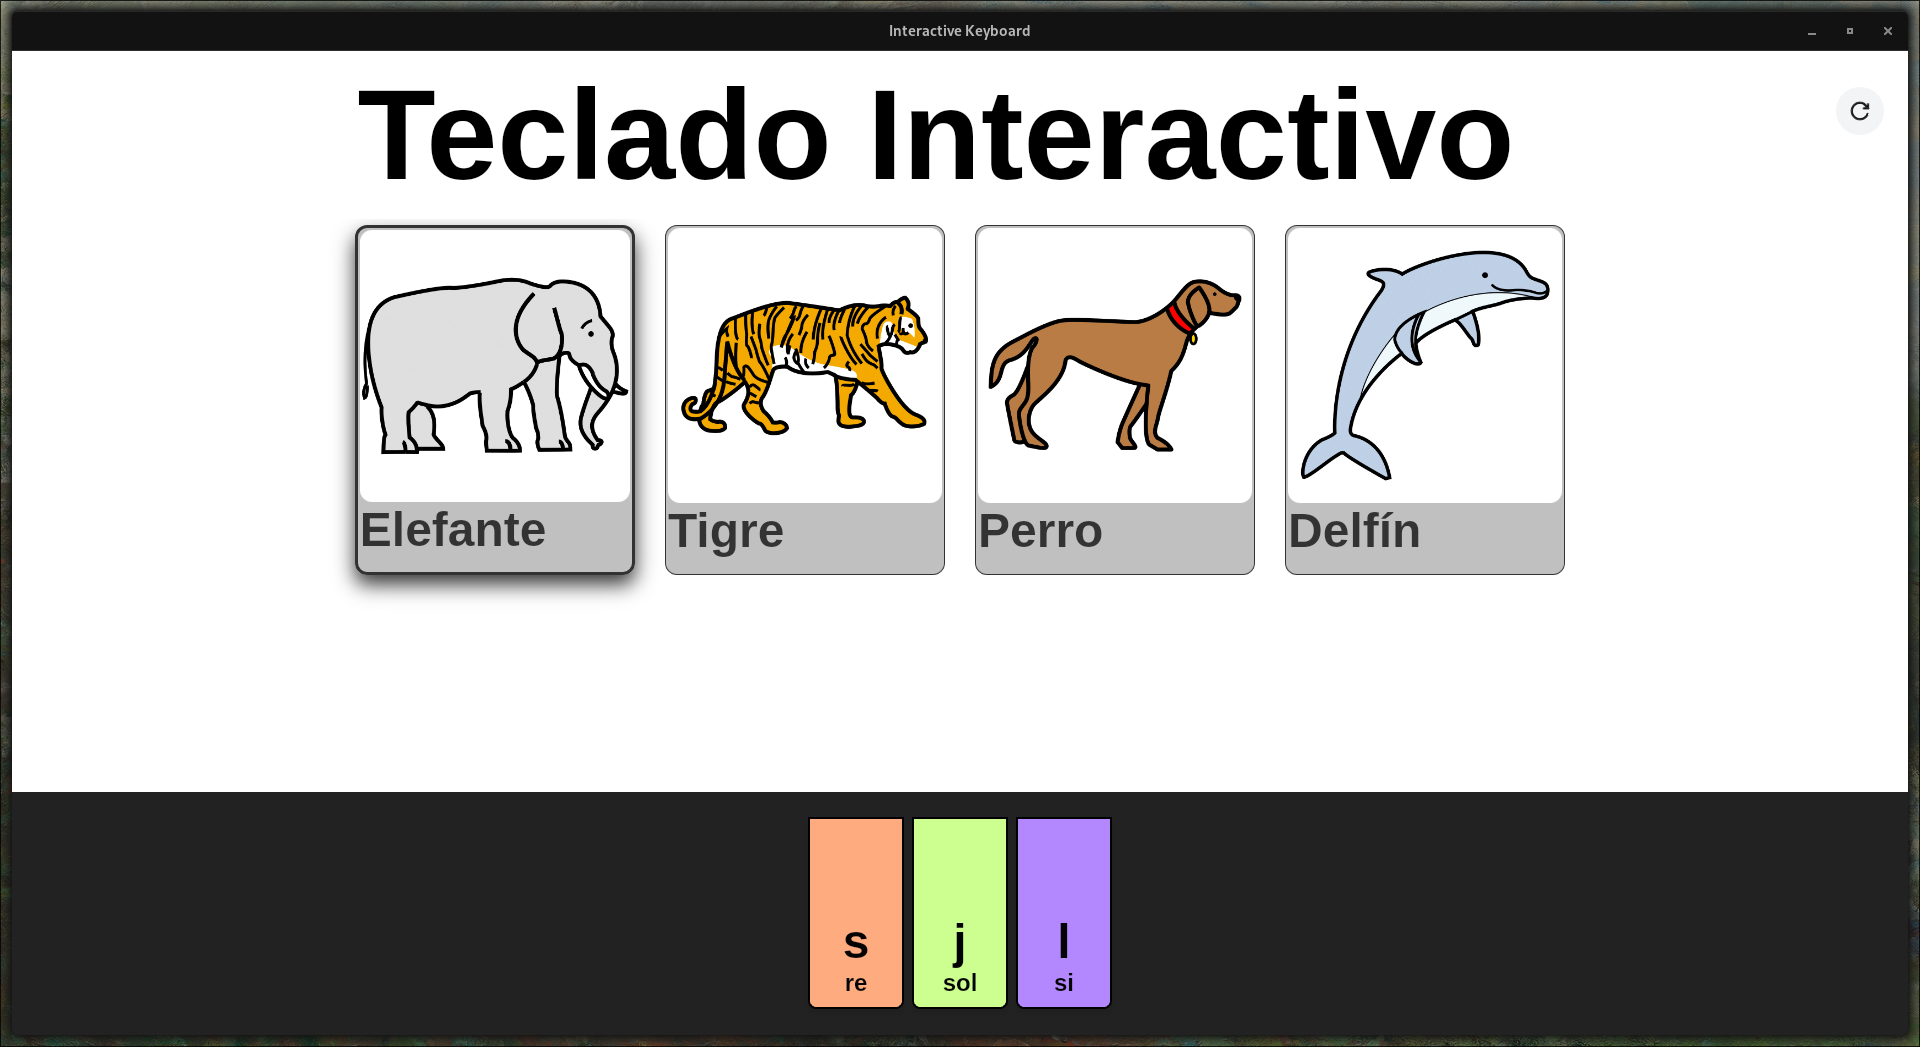
\includegraphics[width=0.75\textwidth]{imaxes/app.png}
  \caption{Deseño final da vista}
  \label{fig:app}
\end{figure}

Unha vez rematado o desenvolvemento propiamente dito, procedeuse cunha fase de probas. Dada a natureza en tempo real da aplicación o máis sinxelo foi realizar unha proba manual comprobando o correcto funcionamento de todos os casos de uso da aplicación en todas as plataformas soportadas(Linux e Windows). Para obter de forma sinxela binarios da aplicación para a súa proba nun contexto real creouse unha tarefa de Github Action que permite crear os binarios de produción para varias plataformas sen necesidade de compilación cruzada, como vemos na figura \ref{fig:cd}. Despois, os instaladores producidos publícanse como lanzamentos en Github, permitindo que os usuarios sen coñecementos técnicos instalen a aplicación sen necesidade de instalar as dependencias de desenvolvemento de Tauri.

\begin{figure}[hp!]
  \centering
  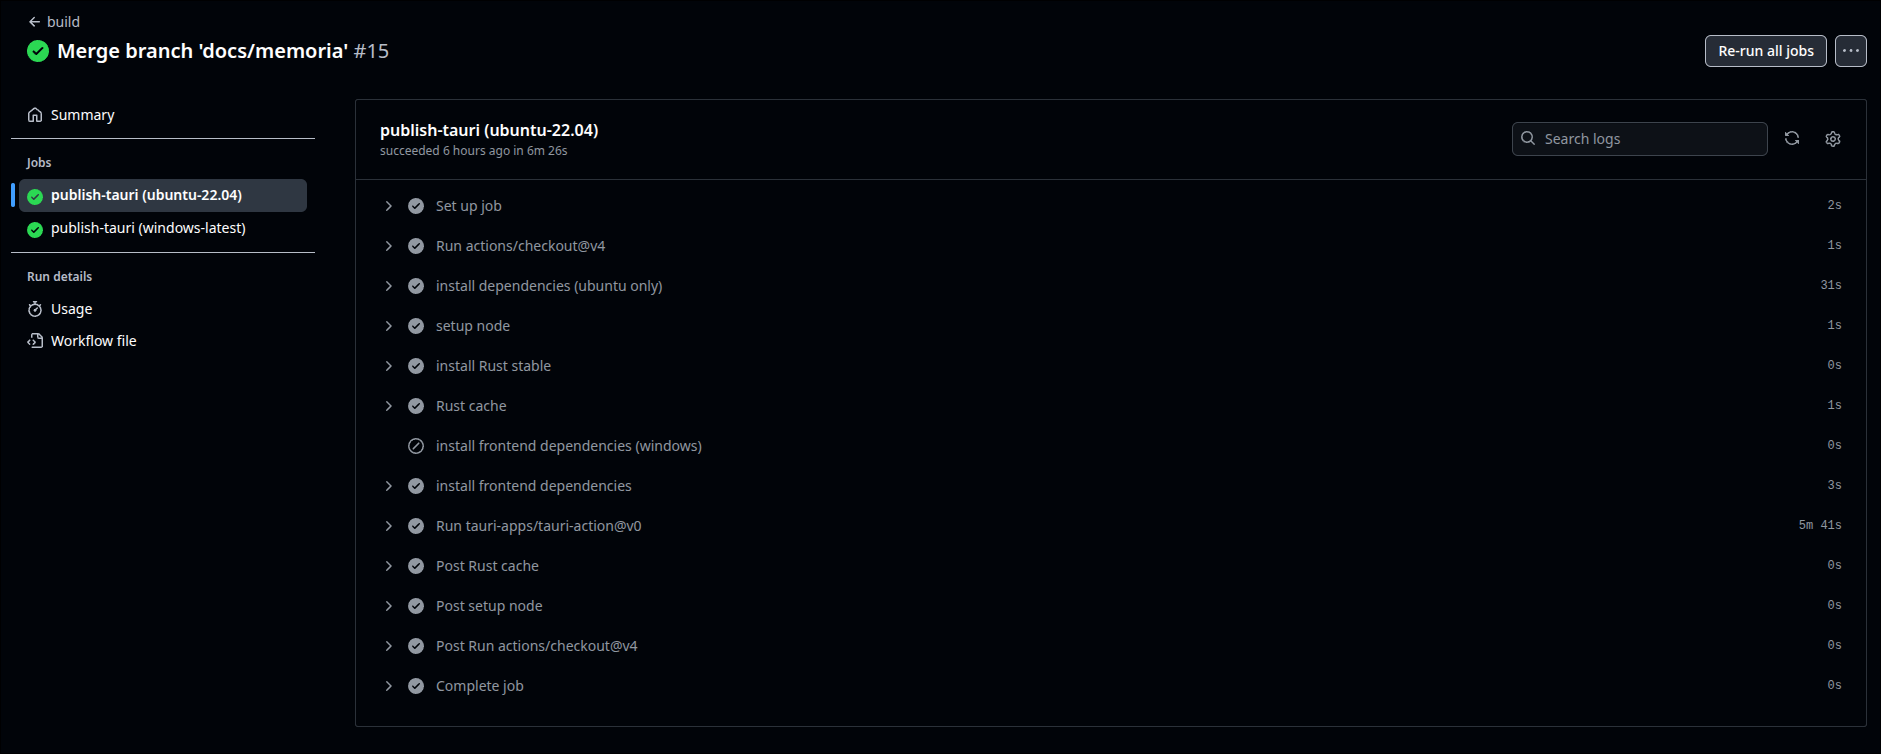
\includegraphics[width=0.75\textwidth]{imaxes/cd.png}
  \caption{Traballos en Github Actions}
  \label{fig:cd}
\end{figure}

% Se puede añadir partes del código que sean importantes para entender el desarrollo.

% Se pueden incluir cuadros (tablas). Los cuadros tienen que estar referenciados en el texto (por ejemplo, el cuadro \ref{tab:exemplo}).
